\documentclass[10pt]{beamer}

\usetheme[]{JuanLesPins}
\setbeamercolor{structure}{fg=brown}
\setbeamertemplate{navigation symbols}{}
\setbeamertemplate{footline}[frame number]
%-------------------------------------------------------
% INCLUDE PACKAGES
%-------------------------------------------------------

\usepackage[utf8]{inputenc}
\usepackage[francais]{babel}
\usepackage[T1]{fontenc}
\usepackage{helvet}
\usepackage{graphicx}
\usepackage{amsmath,amsfonts,amssymb}
\usepackage{enumitem}
\usepackage{float}
\usepackage{hyperref}
\usepackage{cases}

%-------------------------------------------------------
% INFORMATION IN THE TITLE PAGE
%-------------------------------------------------------

\title[Population Néanderthal]{\textbf{Evolution de la population d'Homo Néanderthal}}
\author[Y. Adimy M. Simon H. Vassal]{Y. Adimy M. Simon H. Vassal}
\institute[]{INSA Lyon - Bioinformatique et Modélisation}
\date{13 Juin 2016}
\titlegraphic{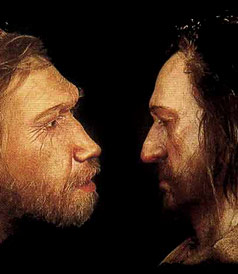
\includegraphics[width=3cm]{neanderthal-sapiens.jpg}}
\logo{
\includegraphics[scale=0.1]{logo_insa.png}}

%-------------------------------------------------------
% THE BODY OF THE PRESENTATION
%-------------------------------------------------------

\begin{document}

%-------------------------------------------------------
% THE TITLEPAGE
%-------------------------------------------------------

\begin{frame}[plain,noframenumbering] 
   \titlepage
   \insertlogo
\end{frame}

\begin{frame}{Contexte biologique}{}
\end{frame}


%Presentation des modèles
\begin{frame}{Présentation des modèles étudiés}{Cadre général}
\begin{block}{Modèle général}
	\begin{equation}
		\frac{\partial u(t,x)}{\partial t}=f(u(t,x))+d\Delta u(t,x), \quad t \in \mathbb{R}, x \in \mathbb{R}
	\end{equation}
\end{block}
\begin{itemize}
	\item u(t,x) : Densité de population  $\ \in[0,1]$ 
    \item $d$ : Constante de diffusion 
\end{itemize}
\end{frame}

\begin{frame}{Présentation des modèles étudiés}{Croissance logistique}
\begin{block}{Croissance Logistique}
	$$\frac{\partial u(t,x)}{\partial t}=f(u(t,x))+d\Delta u(t,x)$$
	$$f(u(t,x))=\alpha u (1 - \dfrac{u}{K}) $$
\end{block}
\begin{itemize}
    \item $K$ : Capacité de transport 
    \item $\alpha$ : Taux de croissance maximum
\end{itemize}
\end{frame}

\begin{frame}{Présentation des modèles étudiés}{Modèle Allee}
\begin{block}{Modèle Allee}
	$$\frac{\partial u(t,x)}{\partial t}=f(u(t,x))+d\Delta u(t,x)$$
	$$f(u(t,x))=ku(1-u)(u-A)$$
\end{block}
\begin{itemize}
    \item $k$ : Taux de croissance normalisé constant 
    \item $A$ : Densité critique
\end{itemize}
$$k=\frac{4}{(1-A)^2}$$
\end{frame}

\begin{frame}{Présentation des modèles étudiés}{Système de Lotka-Volterra}
\begin{block}{Modèle de compétition}
	$$\begin{cases} \frac{\partial u(t,x)}{\partial t} = f(u,v) + d_1\Delta u\\ \frac{\partial v(t,x)}{\partial t} = g(u,v) + d_2 \Delta v \\ 
\end{cases}$$
	$$f(u,v) = \alpha_1 u\left(1-\frac{u}{K_1}-\gamma_1\frac{v}{K_1}\right) \text{, } g(u,v) = \alpha_2 v\left(1-\frac{v}{K_2}-\gamma_2\frac{u}{K_2}\right)$$
\end{block}
\begin{itemize}
	\item u(t,x) : Densité de population des Hommes Modernes 
    \item v(t,x) : Densité de population des Hommes de Néanderthal 
    \item $K_1$ et $K_2$ : Capacités d'accueil du milieu
    \item $\gamma_1$ et $\gamma_2$ : Coefficients de compétition
    \item $\alpha_1$ et $\alpha_2$ : Taux de croissance
\end{itemize}
\end{frame}

%Analyse mathématiques
%%Croissance logistique
\begin{frame}{Analyse mathématique}{Croissance logistique}
\begin{itemize}
	\item[$\bullet$] Équilibres: $u=0 {\ et\ } u=K$
	\item[$\bullet$] MONOSTABLE
	\item[$\bullet$] Vitesse minimale $c_0=2\sqrt{\alpha}$
\end{itemize}
\end{frame}

%%effet Allee
\begin{frame}{Analyse mathématique}{Effet Allee}
\begin{itemize}
	\item[$\bullet$] Équilibres: $u=0, u=A \text{ et } u=1$
	\item[$\bullet$] BISTABLE
	\item[$\bullet$] 2 scénarios selon la valeur de A :
	\begin{itemize}
		\item[-] $A<0.5$ : $c>0$ $\rightarrow$ "1 envahit 0"
		\item[-] $A>0.5$ : $c<0$ $\rightarrow$ "0 envahit 1"
	\end{itemize}
\end{itemize}
\end{frame}

%%Competition
\begin{frame}{Analyse mathématique}{Système de Lolkta Volterra}
\end{frame}

%Simulations numeriques
%%Croissance logistique
\begin{frame}{Simulations Numériques}{Croissance logistique}
\end{frame}

%% Effet Allee
\begin{frame}{Simulations Numériques}{Modèle Allee : $\ d=0.5, A=0.25 (k=64), u_0=0.1$}
\begin{figure}[H]
	\centering
	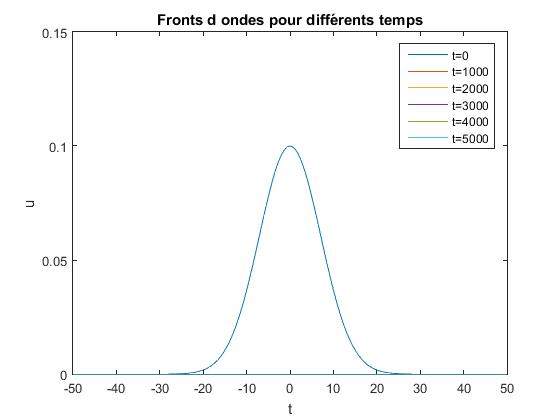
\includegraphics[width=0.40\linewidth, height=3cm]{Allee/F2311}\hfill
	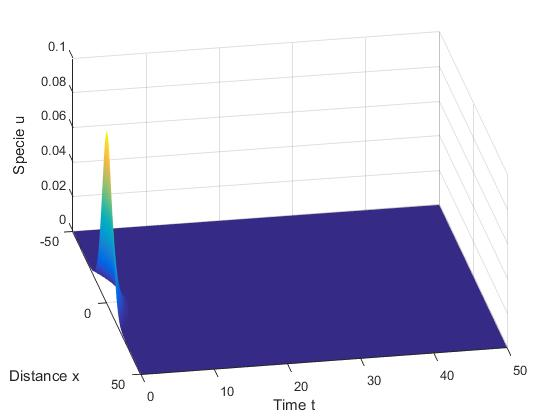
\includegraphics[width=0.55\linewidth, height=3cm]{Allee/F4311}
\end{figure}
\begin{figure}[H]
	\centering
	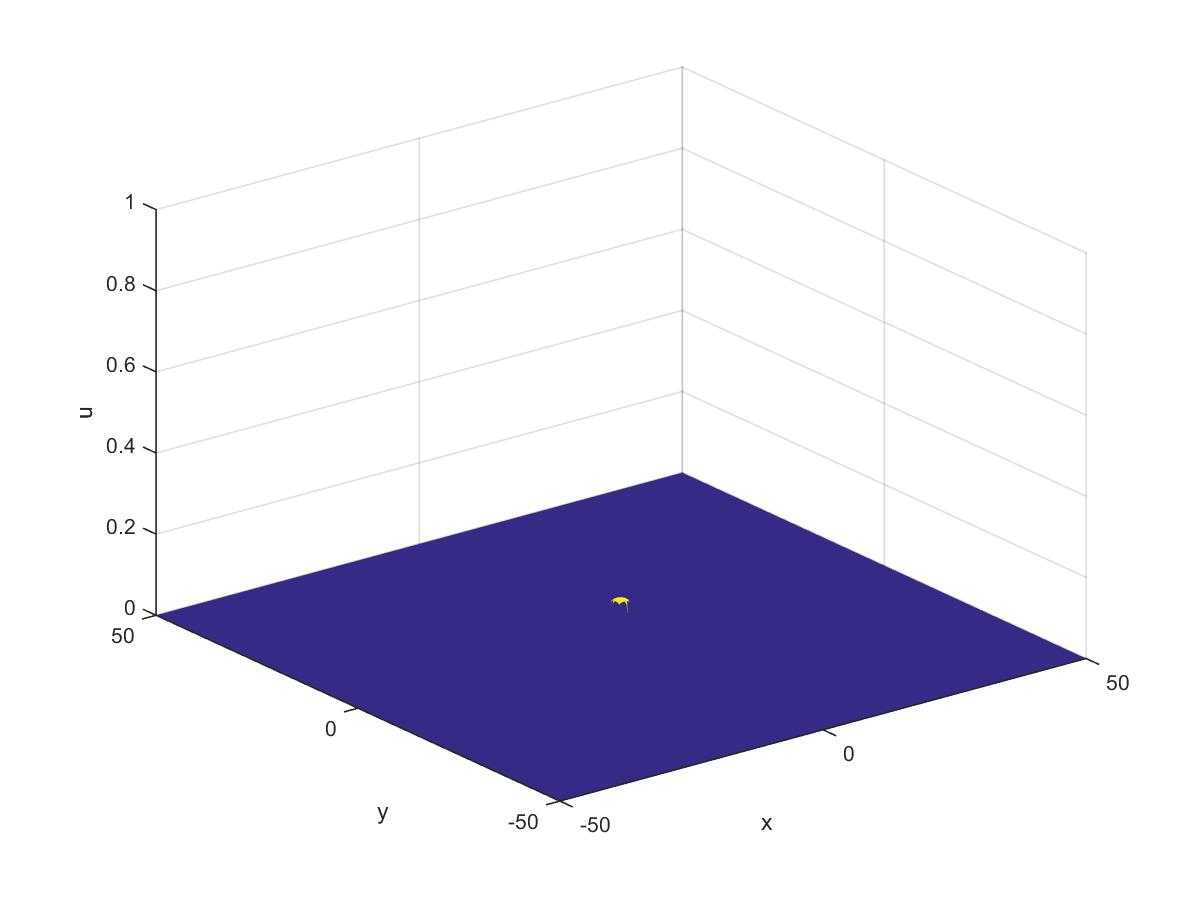
\includegraphics[width=0.3\linewidth]{Allee/311__1_}\hfill
    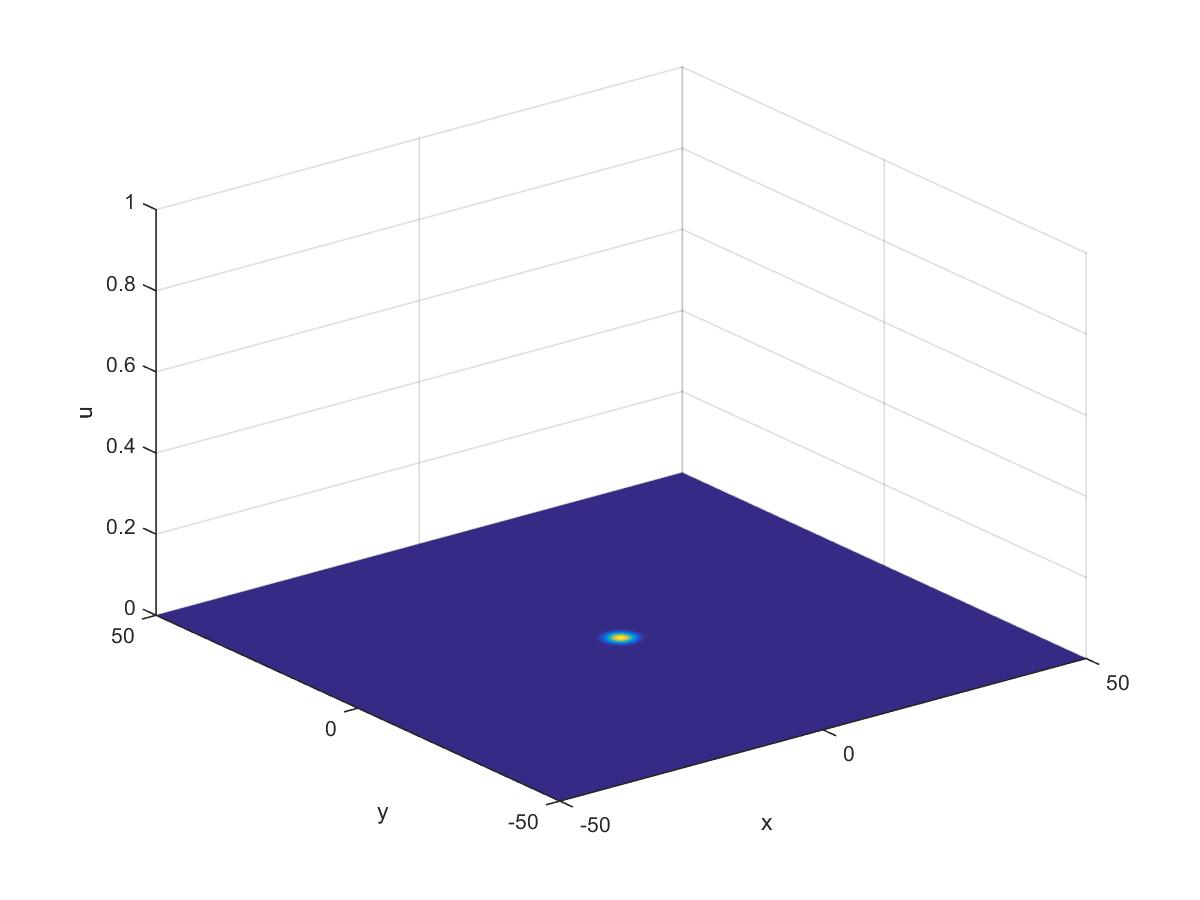
\includegraphics[width=0.3\linewidth]{Allee/311__2_}\hfill
	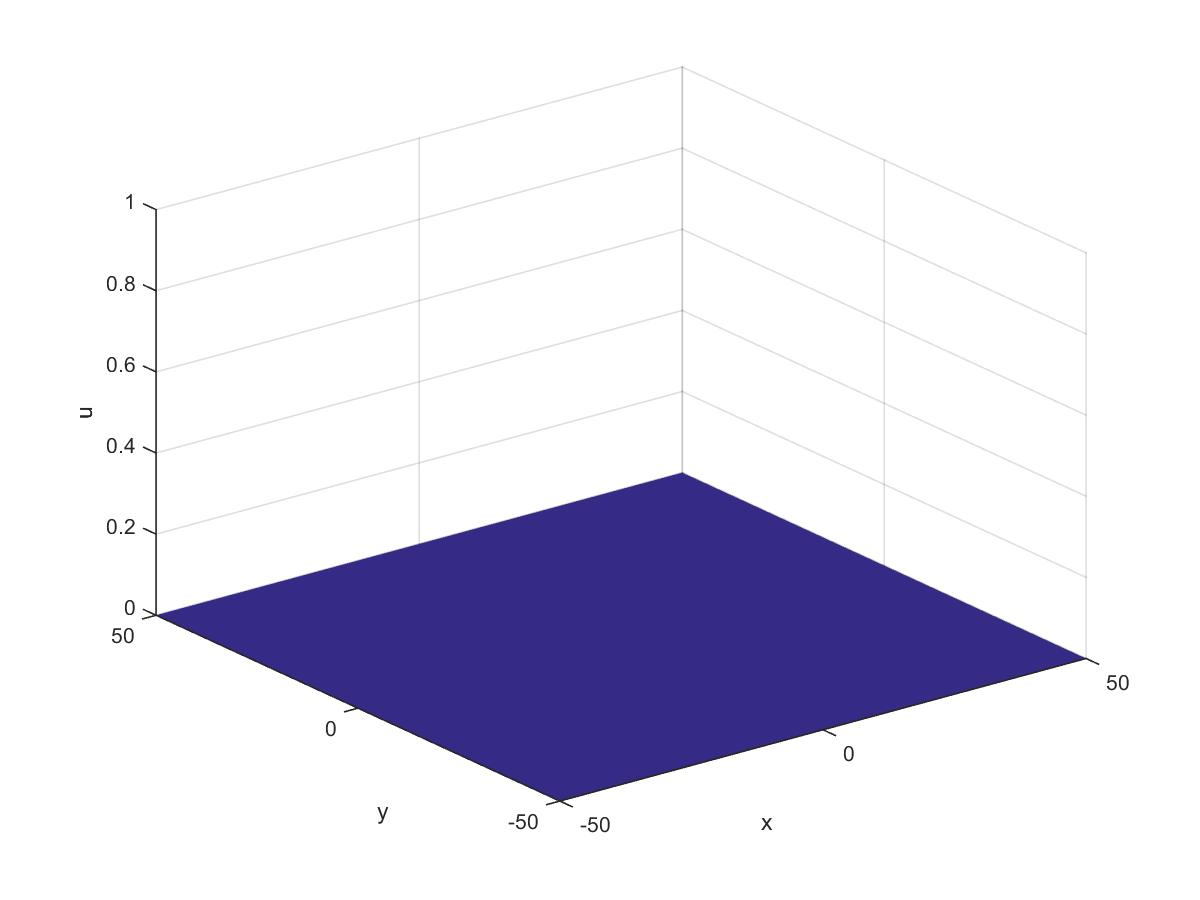
\includegraphics[width=0.3\linewidth]{Allee/311__3_}
\end{figure}
\end{frame}

\begin{frame}{Simulations Numériques}{Modèle Allee : $\ d=0.5, A=0.25 (k=64), u_0=0.5$}
\begin{figure}[H]
	\centering
	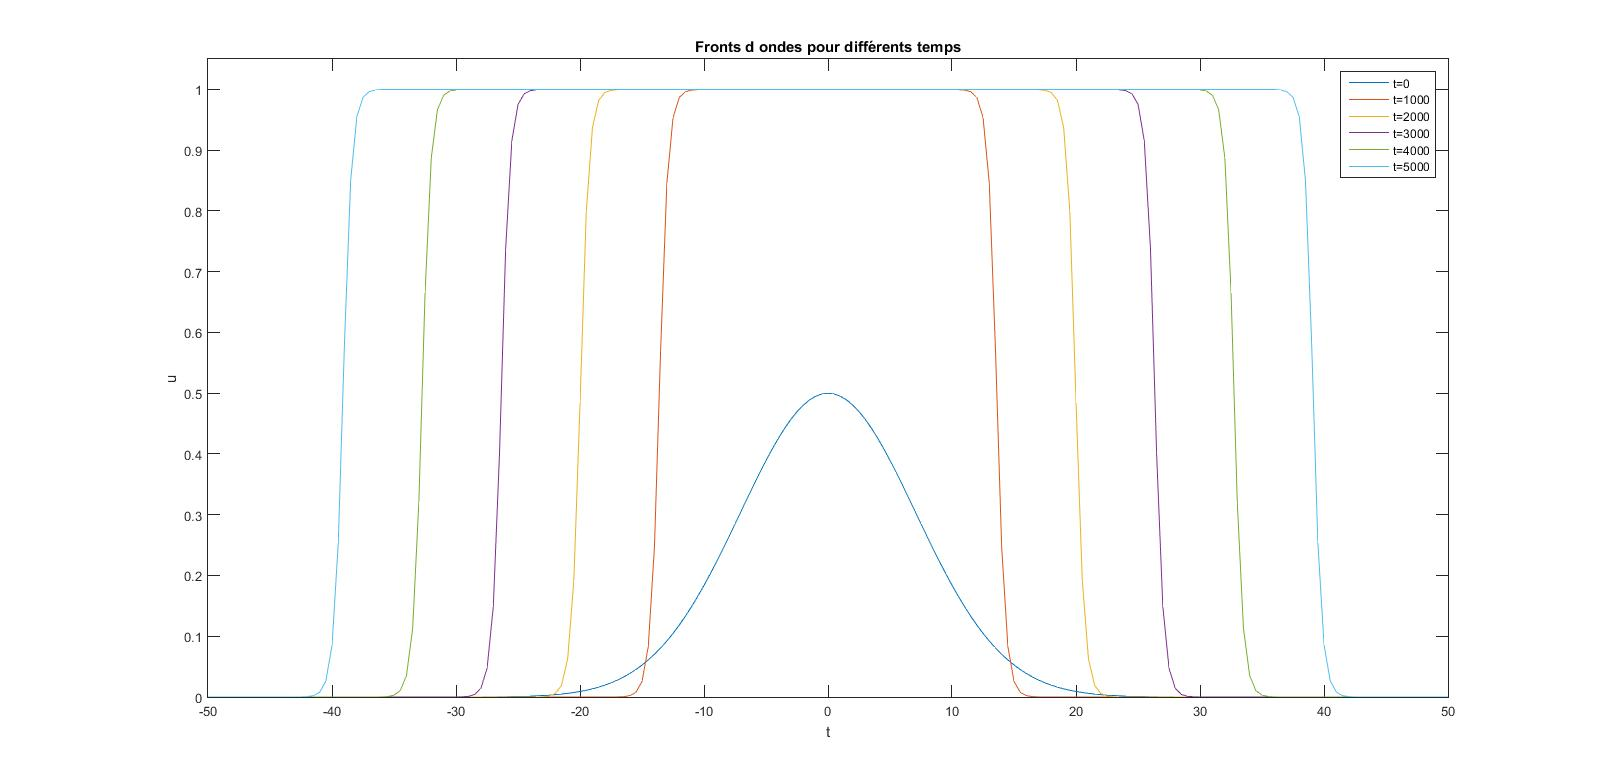
\includegraphics[width=0.40\linewidth, height=3cm]{Allee/F2312}\hfill
	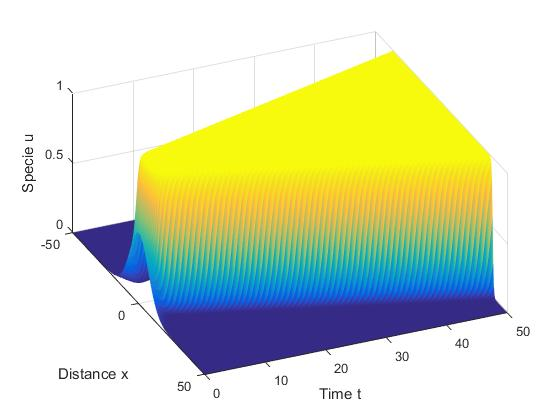
\includegraphics[width=0.55\linewidth, height=3cm]{Allee/F4312}
\end{figure}
\begin{figure}[H]
	\centering
	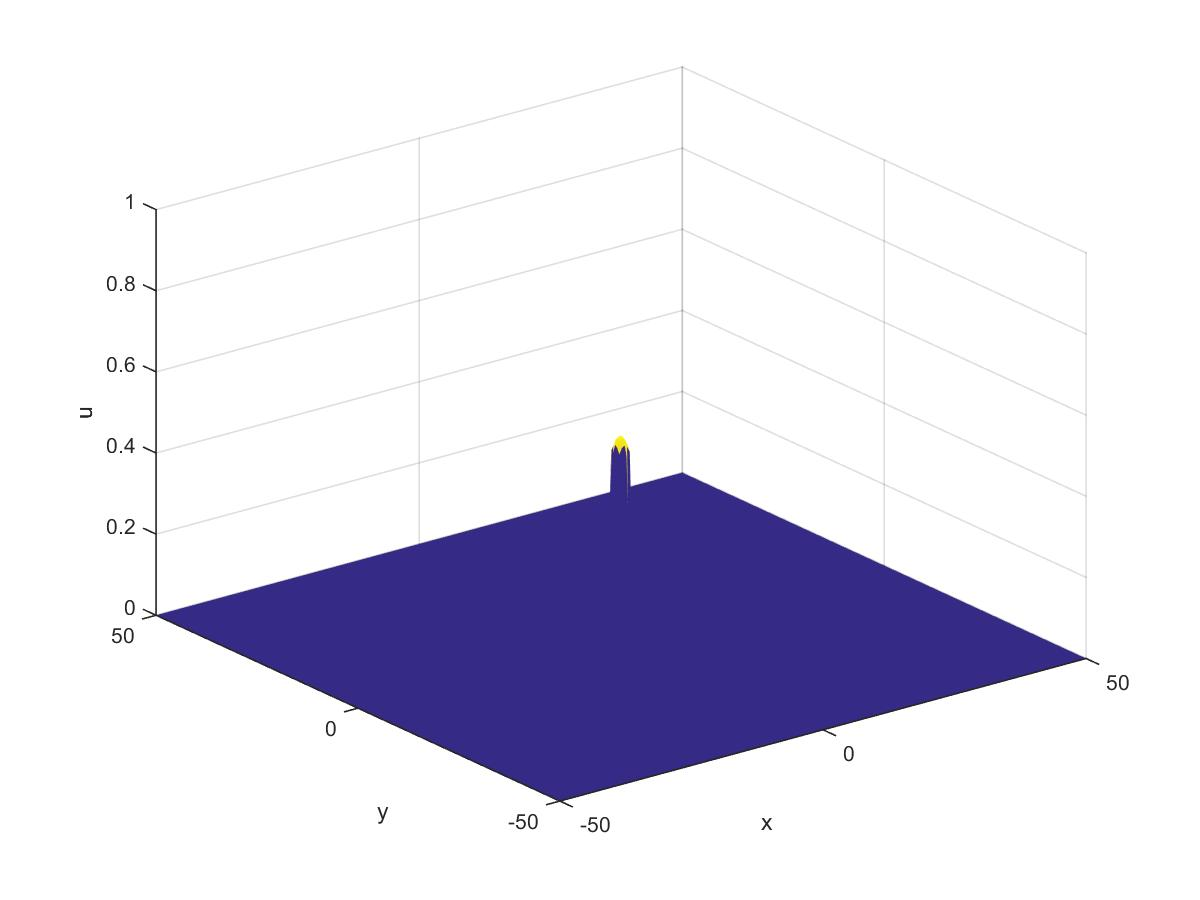
\includegraphics[width=0.3\linewidth]{Allee/312__1_}\hfill
    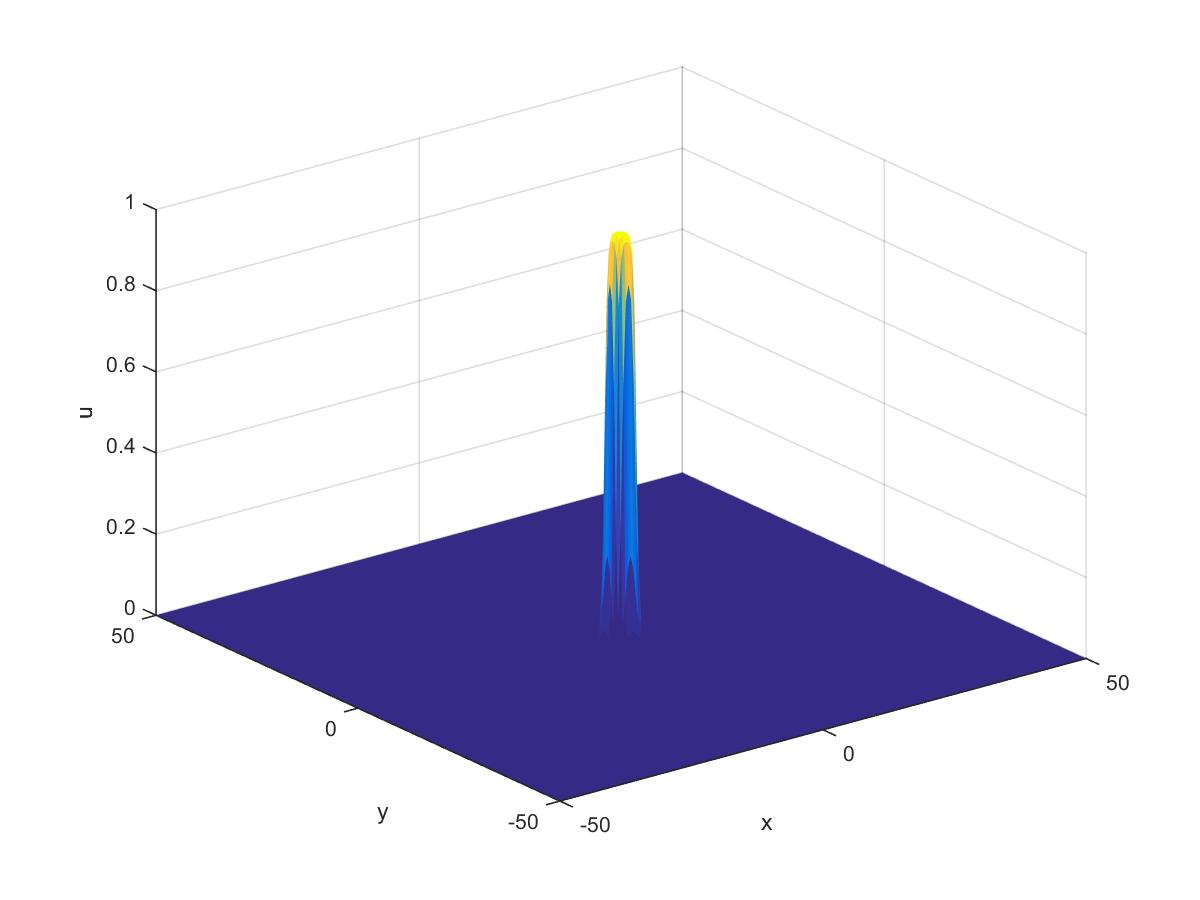
\includegraphics[width=0.3\linewidth]{Allee/312__2_}\hfill
	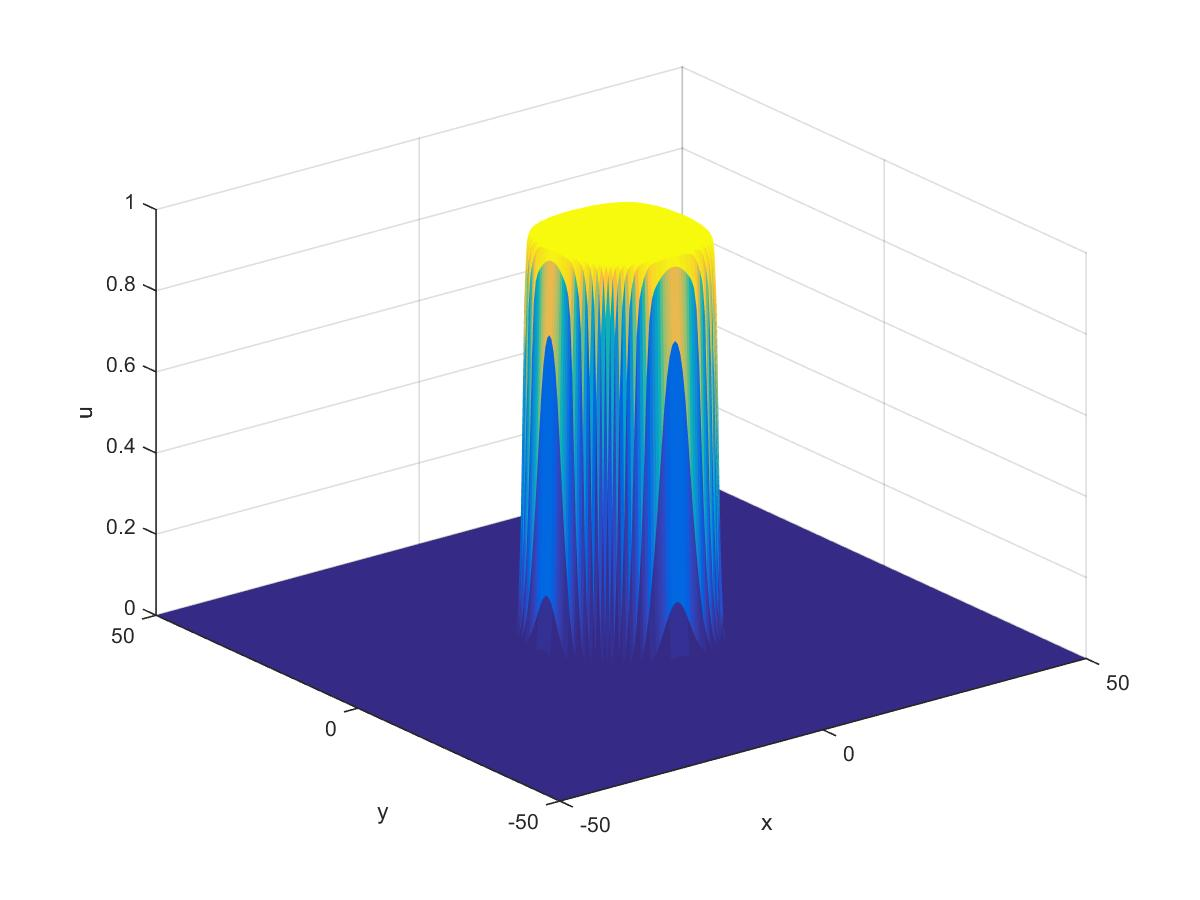
\includegraphics[width=0.3\linewidth]{Allee/312__3_}
\end{figure}
\end{frame}

\begin{frame}{Simulations Numériques}{Modèle Allee : $\ d=0.5, A=0.75 (k=7.1), u_0=0.5$}
\begin{figure}[H]
	\centering
	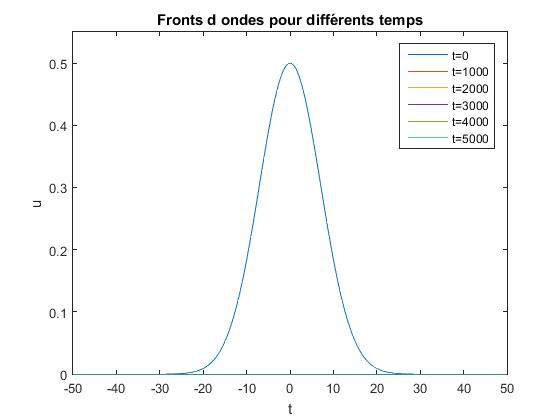
\includegraphics[width=0.40\linewidth, height=3cm]{Allee/F2322}\hfill
	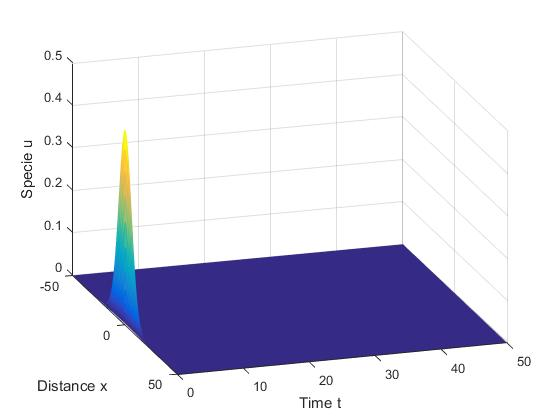
\includegraphics[width=0.55\linewidth, height=3cm]{Allee/F4322}
\end{figure}
\begin{figure}[H]
	\centering
	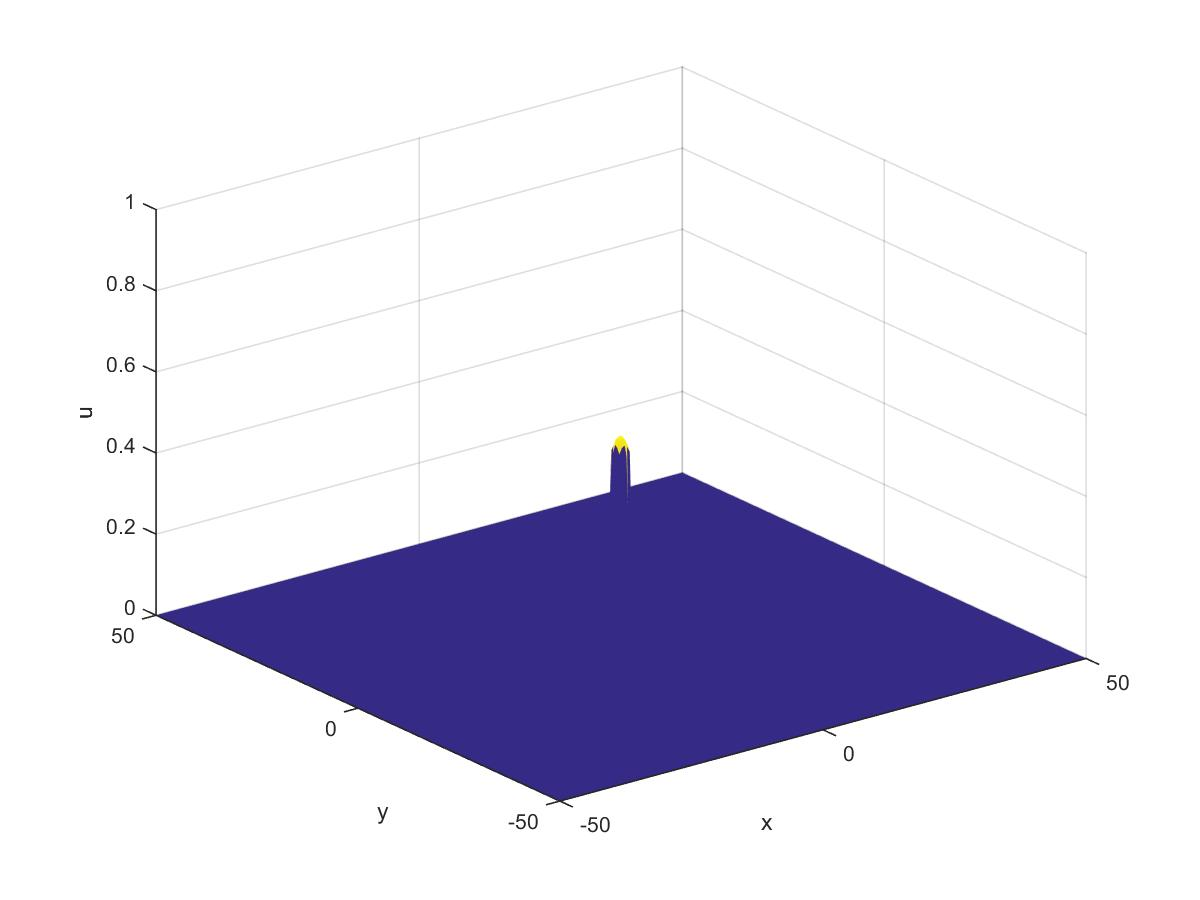
\includegraphics[width=0.3\linewidth]{Allee/322__1_}\hfill
    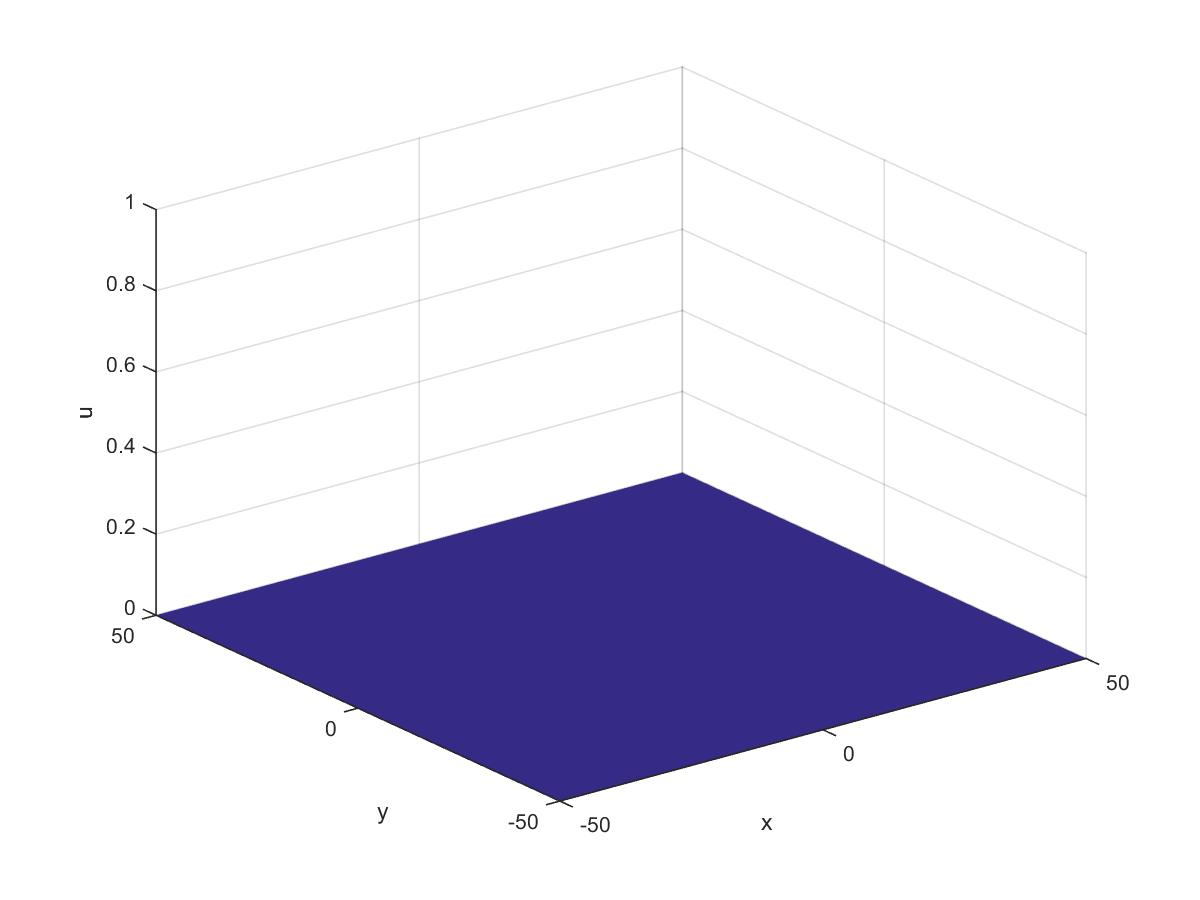
\includegraphics[width=0.3\linewidth]{Allee/322__2_}\hfill
	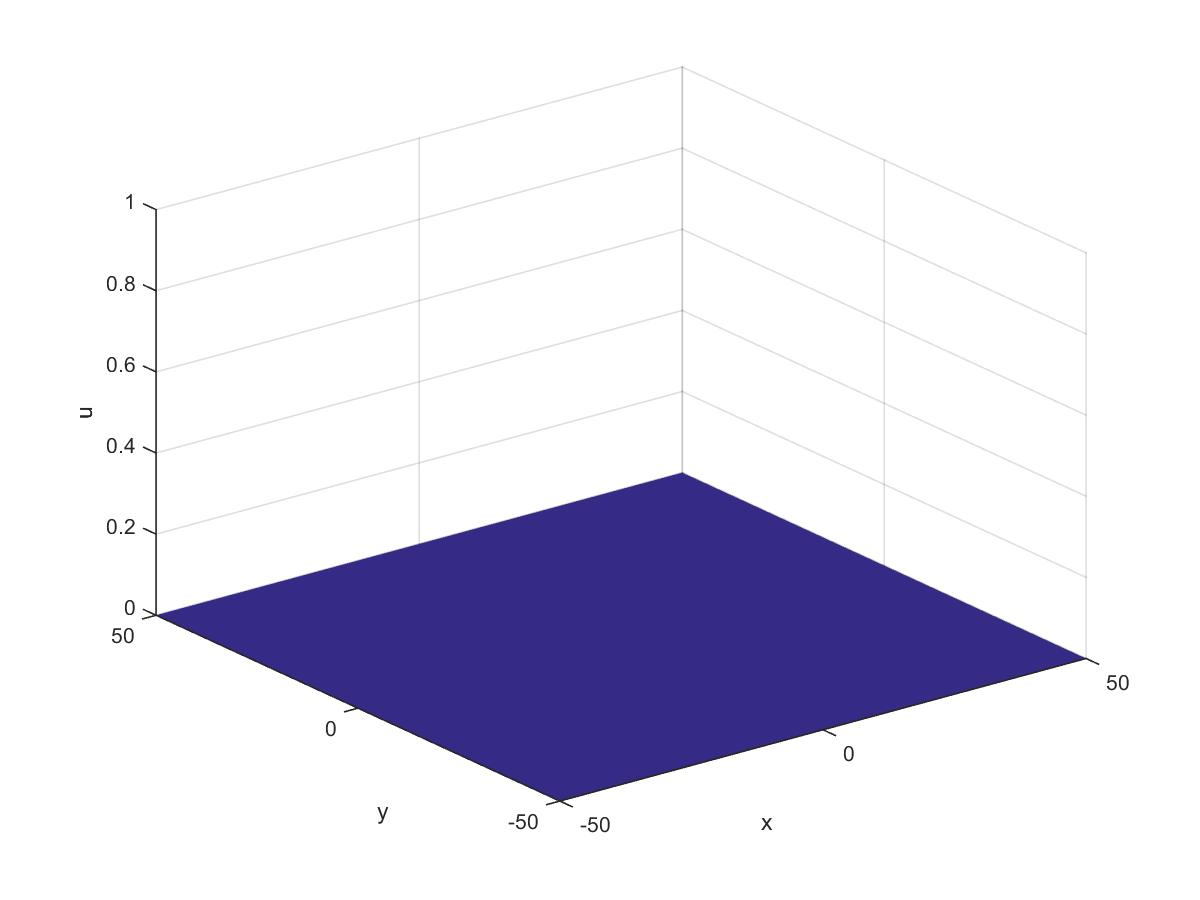
\includegraphics[width=0.3\linewidth]{Allee/322__3_}
\end{figure}
\end{frame}

\begin{frame}{Simulations Numériques}{Modèle Allee : $\ d=0.5, A=0.75 (k=7.1), u_0=0.9$}
\begin{figure}[H]
	\centering
	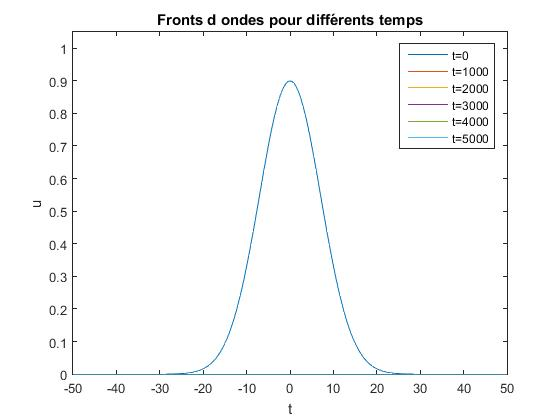
\includegraphics[width=0.40\linewidth, height=3cm]{Allee/F2323}\hfill
	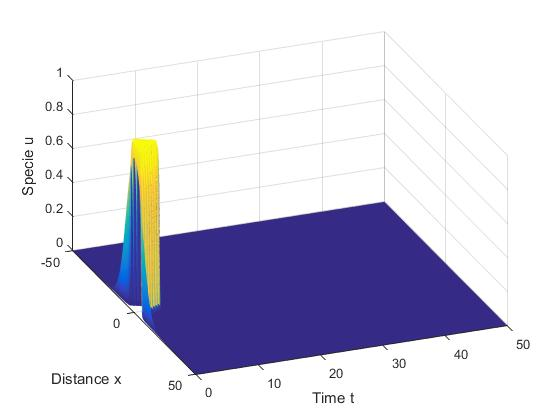
\includegraphics[width=0.55\linewidth, height=3cm]{Allee/F4323}
\end{figure}
\begin{figure}[H]
	\centering
	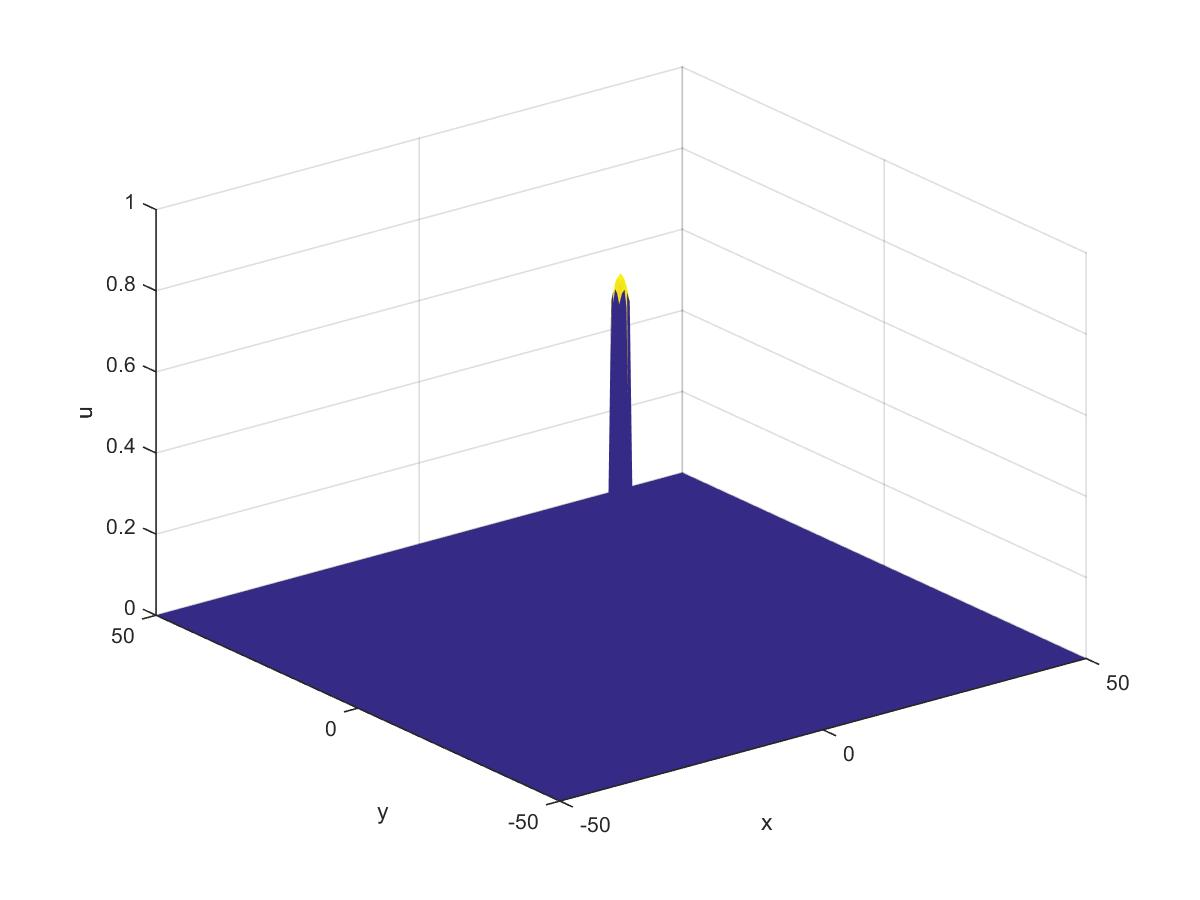
\includegraphics[width=0.3\linewidth]{Allee/323__1_}\hfill
    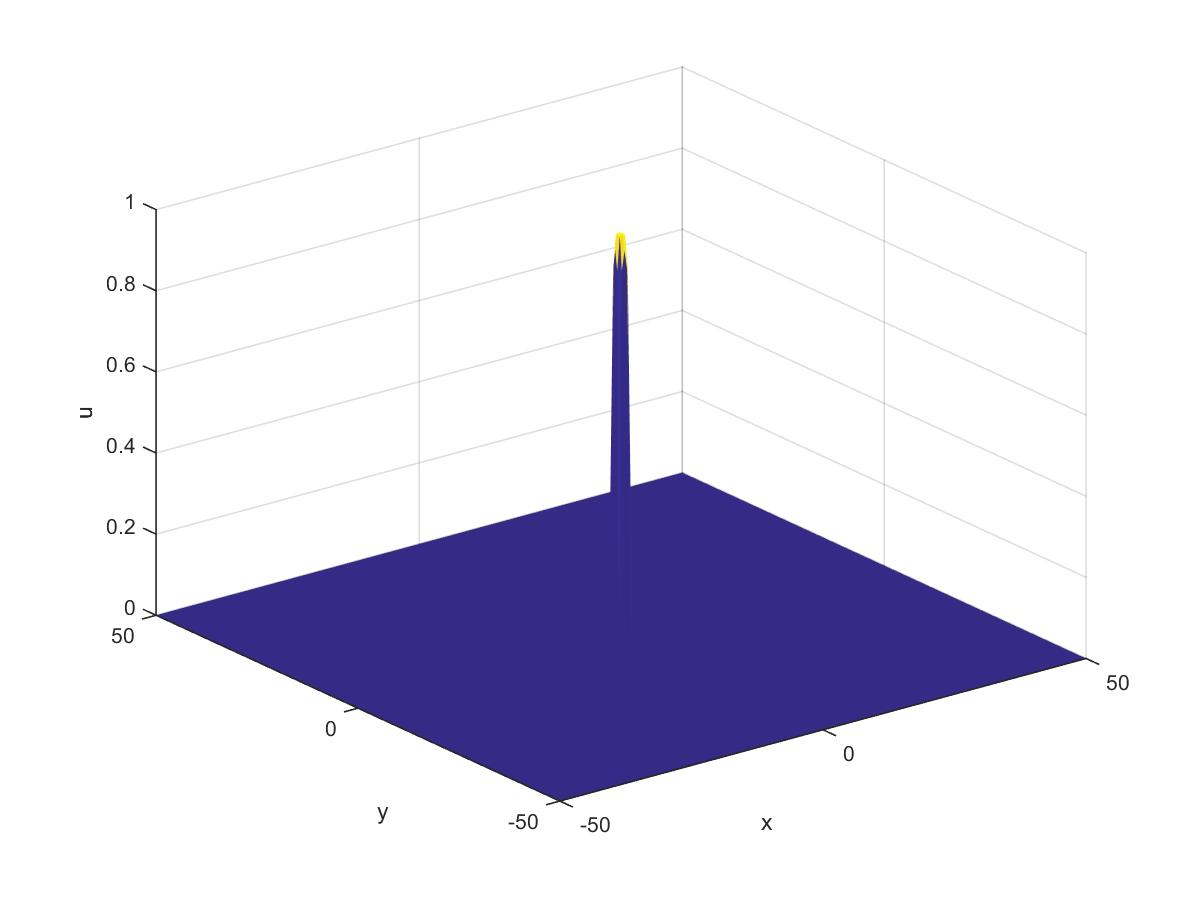
\includegraphics[width=0.3\linewidth]{Allee/323__2_}\hfill
	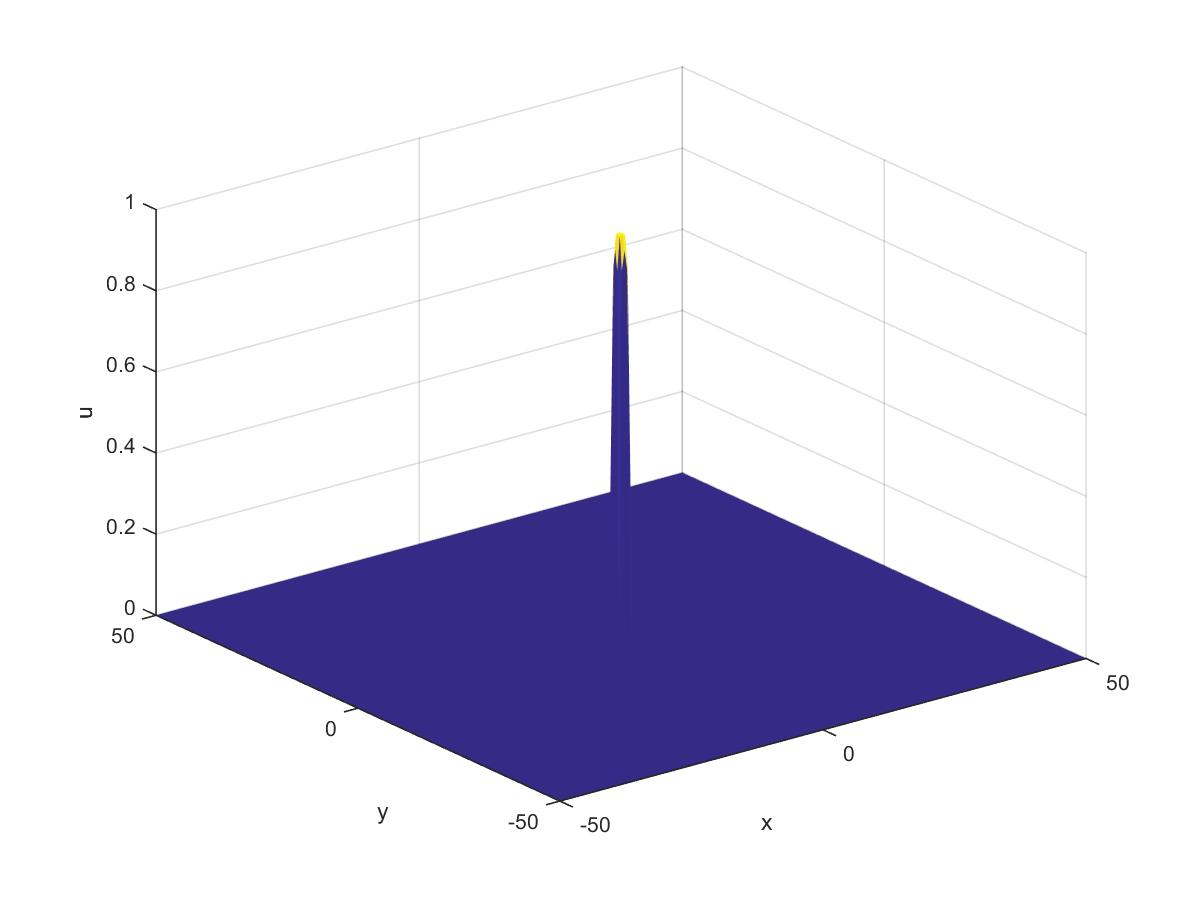
\includegraphics[width=0.3\linewidth]{Allee/323__3_}
\end{figure}
\end{frame}

\begin{frame}{Simulations Numériques}{Modèle Allee :  $\ d=0.5, A=0.5 (k=16), u_0=0.1$}
\begin{figure}[H]
	\centering
	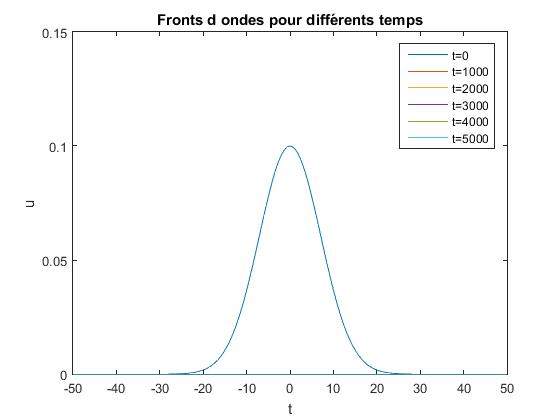
\includegraphics[width=0.40\linewidth, height=3cm]{Allee/F2331}\hfill
	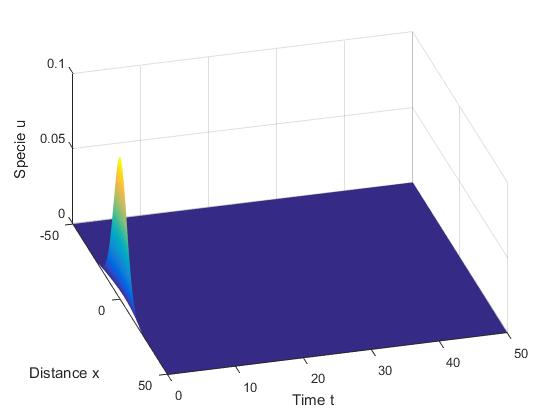
\includegraphics[width=0.55\linewidth, height=3cm]{Allee/F4331}
\end{figure}
\begin{figure}[H]
	\centering
	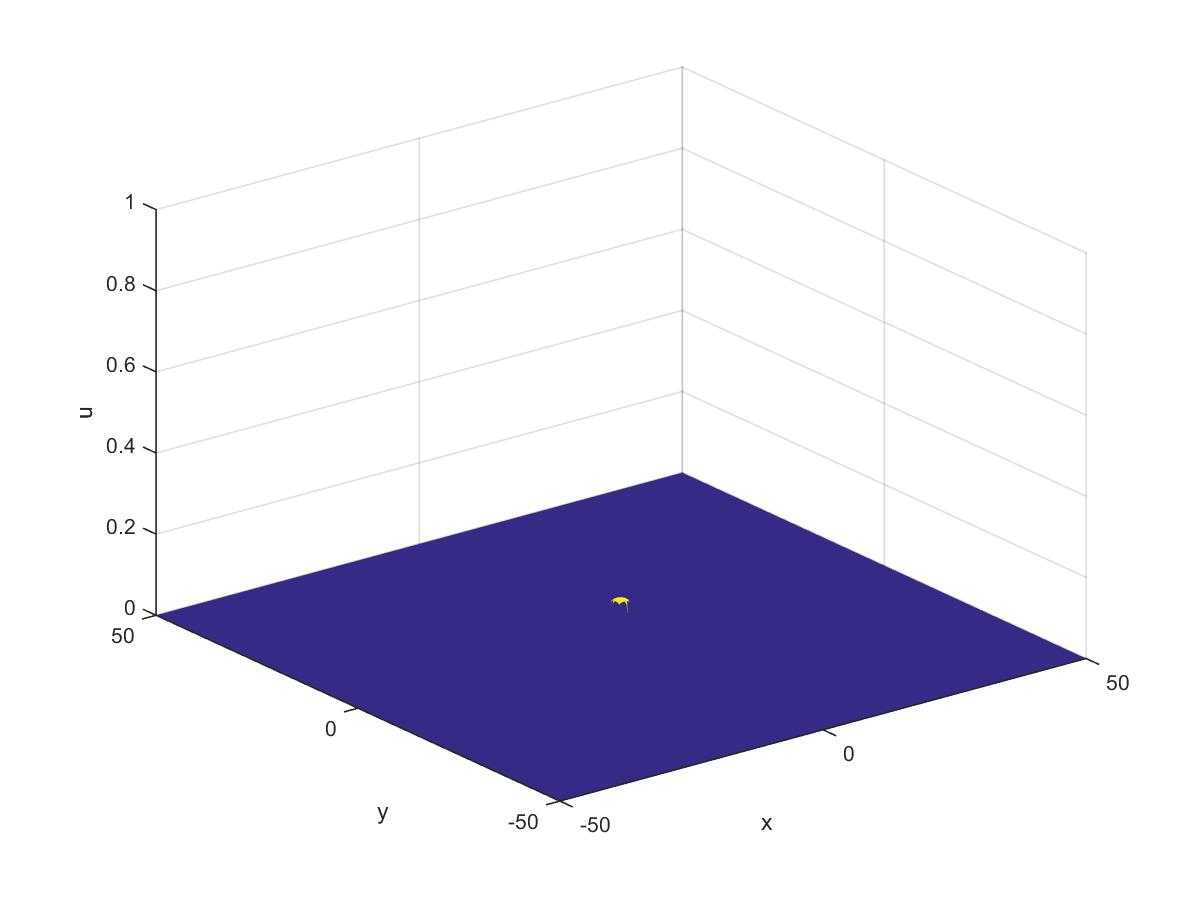
\includegraphics[width=0.3\linewidth]{Allee/331__1_}\hfill
    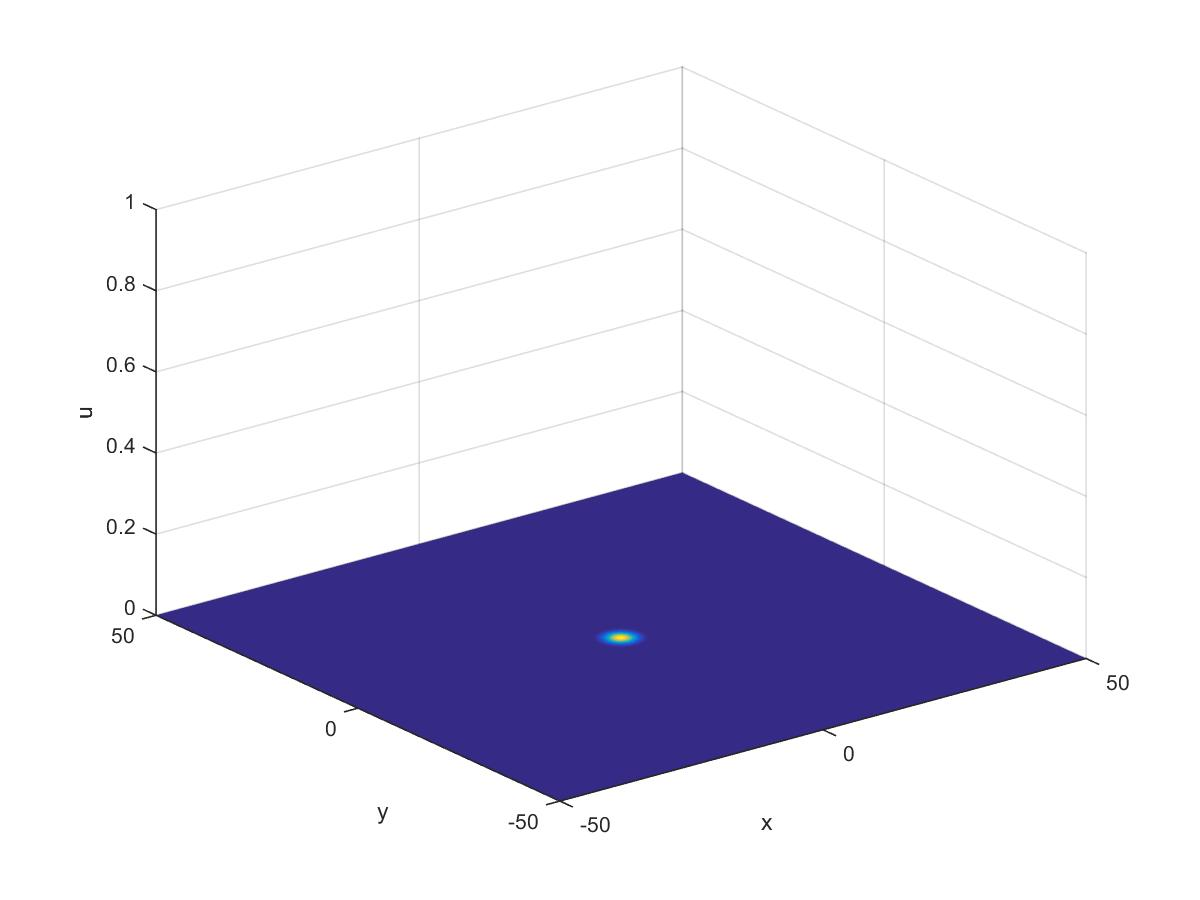
\includegraphics[width=0.3\linewidth]{Allee/331__2_}\hfill
	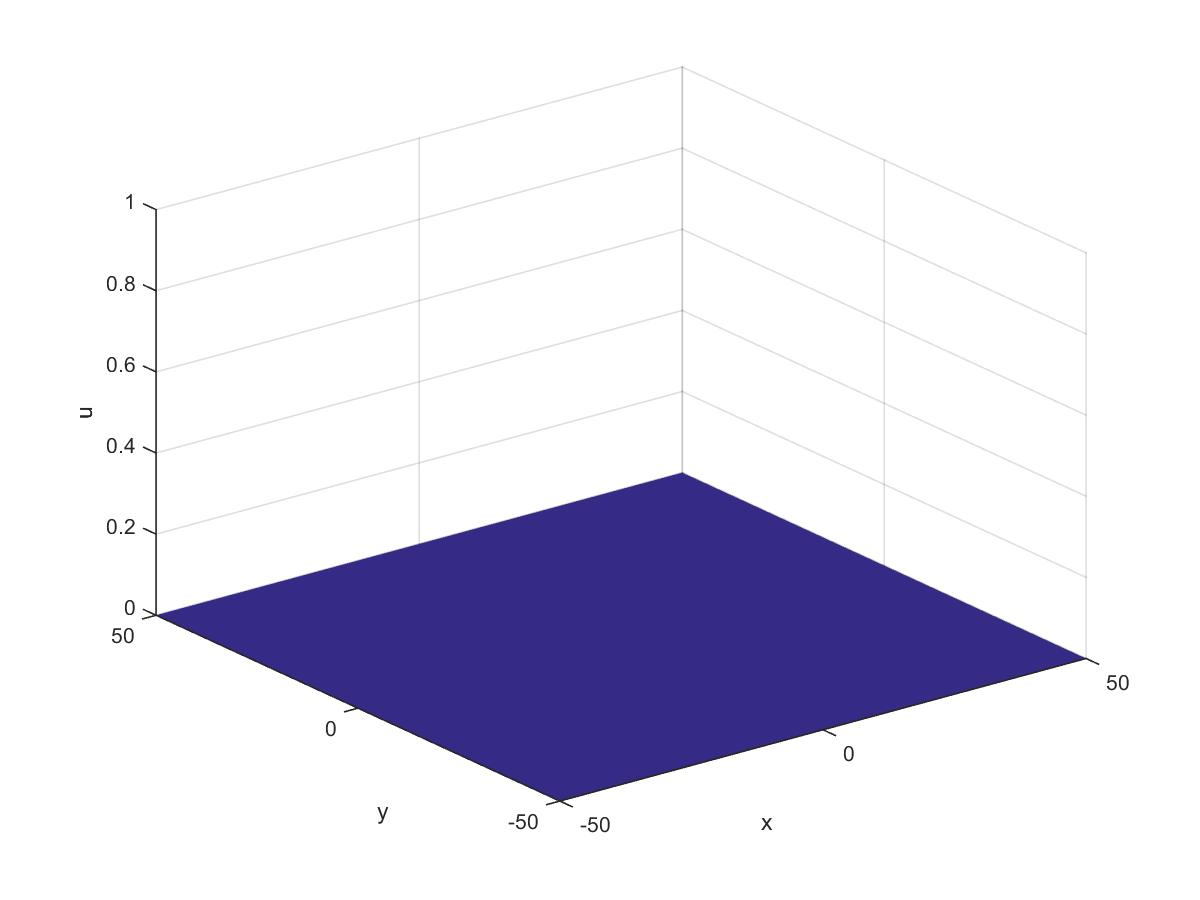
\includegraphics[width=0.3\linewidth]{Allee/331__3_}
\end{figure}
\end{frame}

\begin{frame}{Simulations Numériques}{Modèle Allee :$\ d=0.5, A=0.5 (k=16), u_0=0.9$}
\begin{figure}[H]
	\centering
	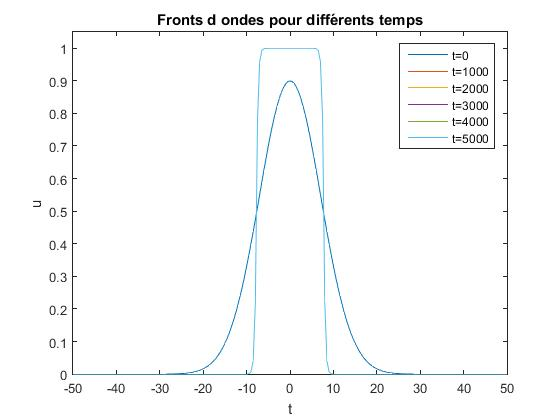
\includegraphics[width=0.40\linewidth, height=3cm]{Allee/F2333}\hfill
	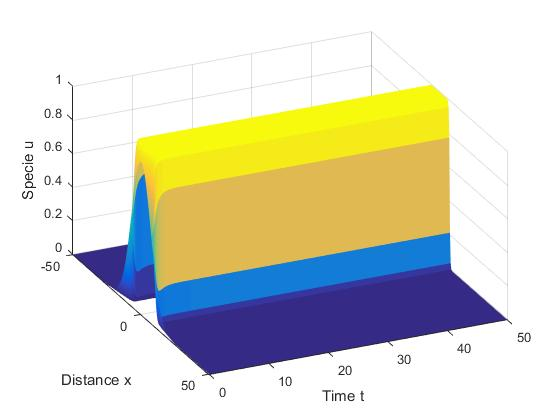
\includegraphics[width=0.55\linewidth, height=3cm]{Allee/F4333}
\end{figure}
\begin{figure}[H]
	\centering
	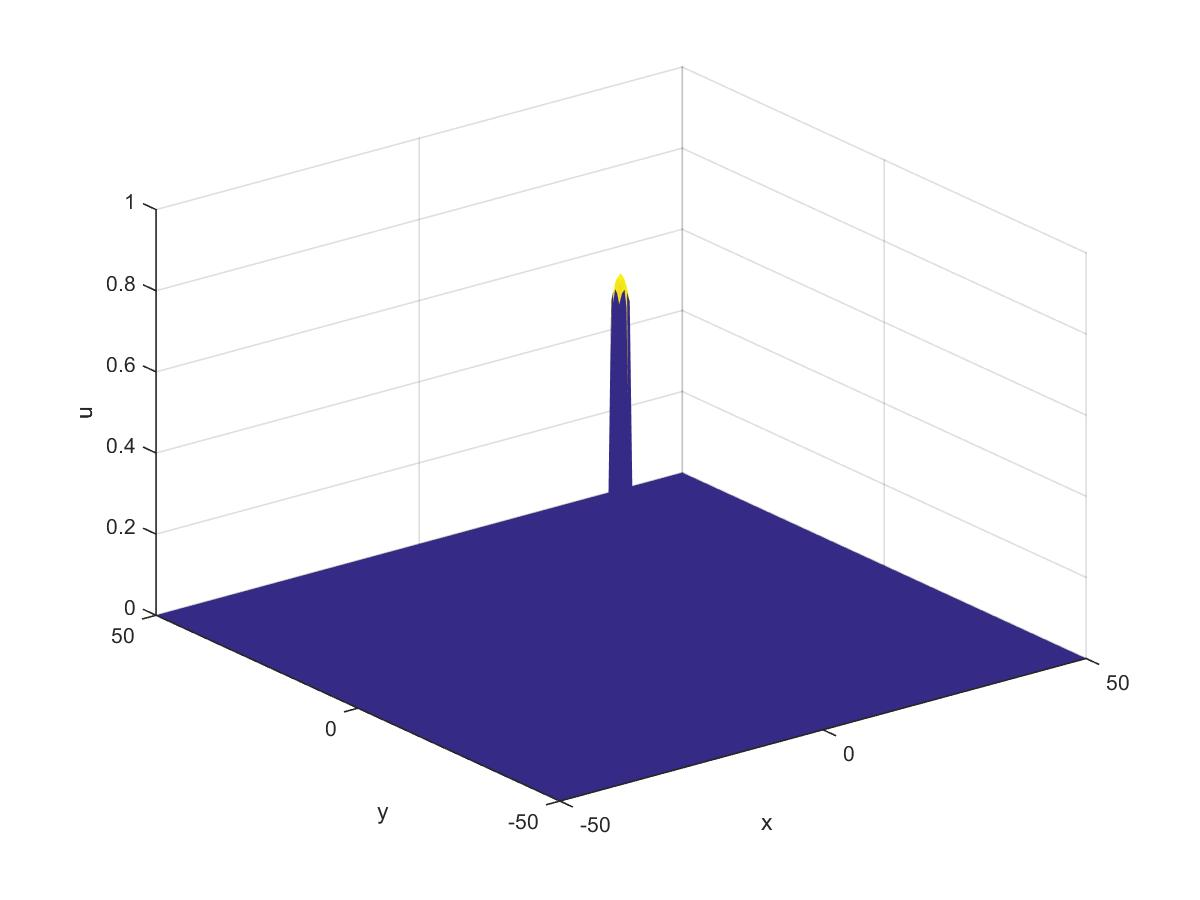
\includegraphics[width=0.3\linewidth]{Allee/333__1_}\hfill
    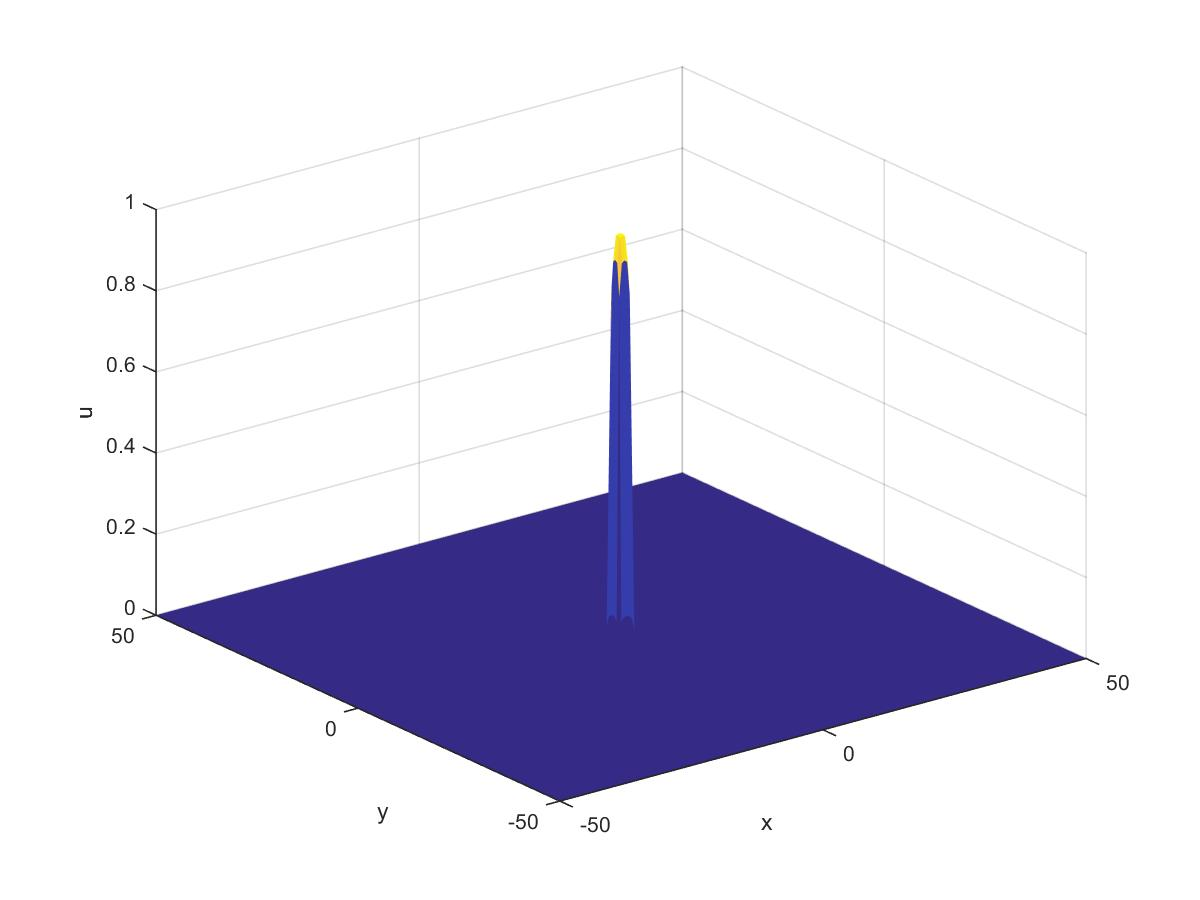
\includegraphics[width=0.3\linewidth]{Allee/333__2_}\hfill
	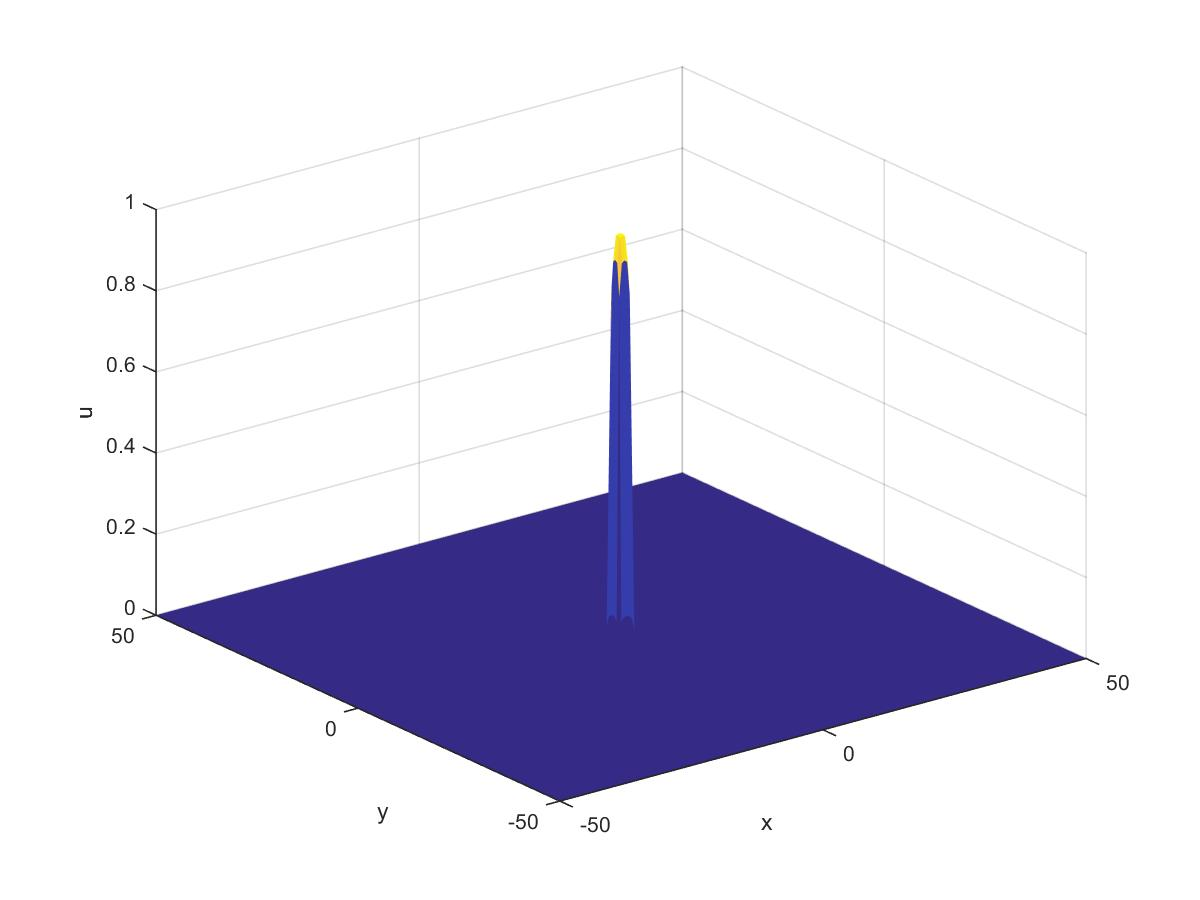
\includegraphics[width=0.3\linewidth]{Allee/333__3_}
\end{figure}
\end{frame}

%%Competition
\begin{frame}{Simulations Numériques}{Système de Lotka Volterra}
\begin{figure}[H]
\centering
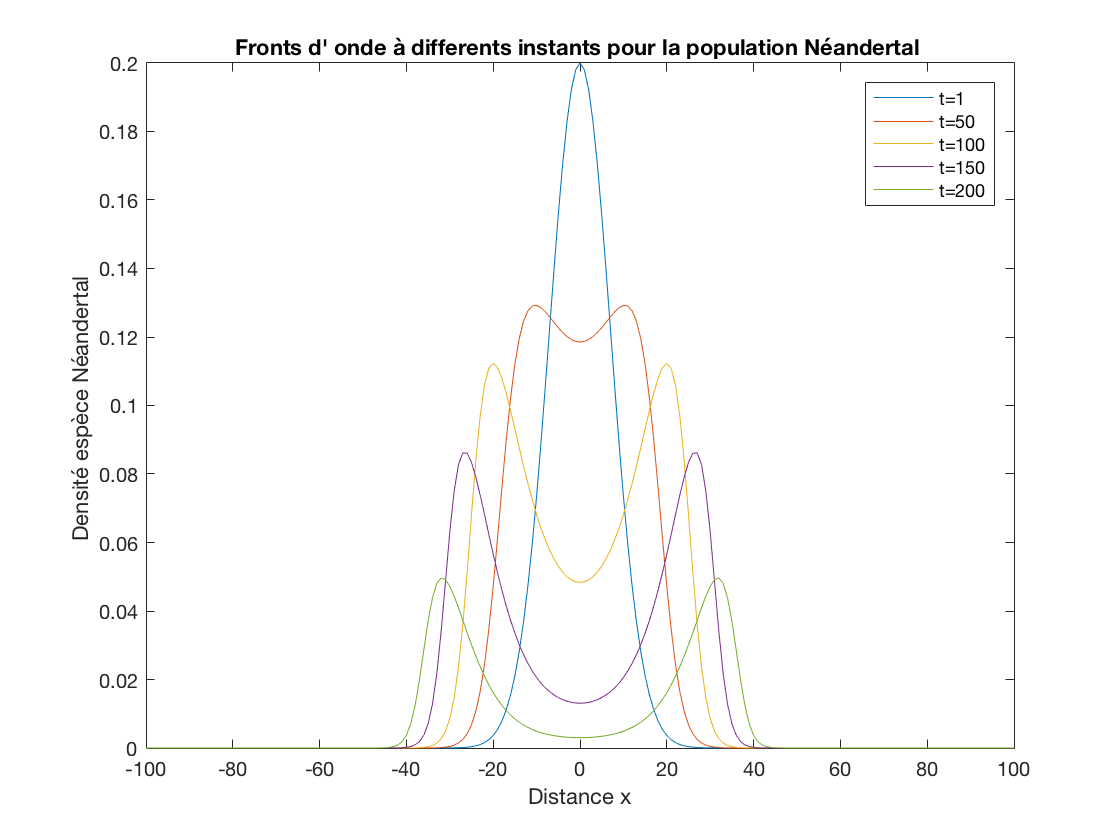
\includegraphics[width=0.48\linewidth]{Comp/neand.png}
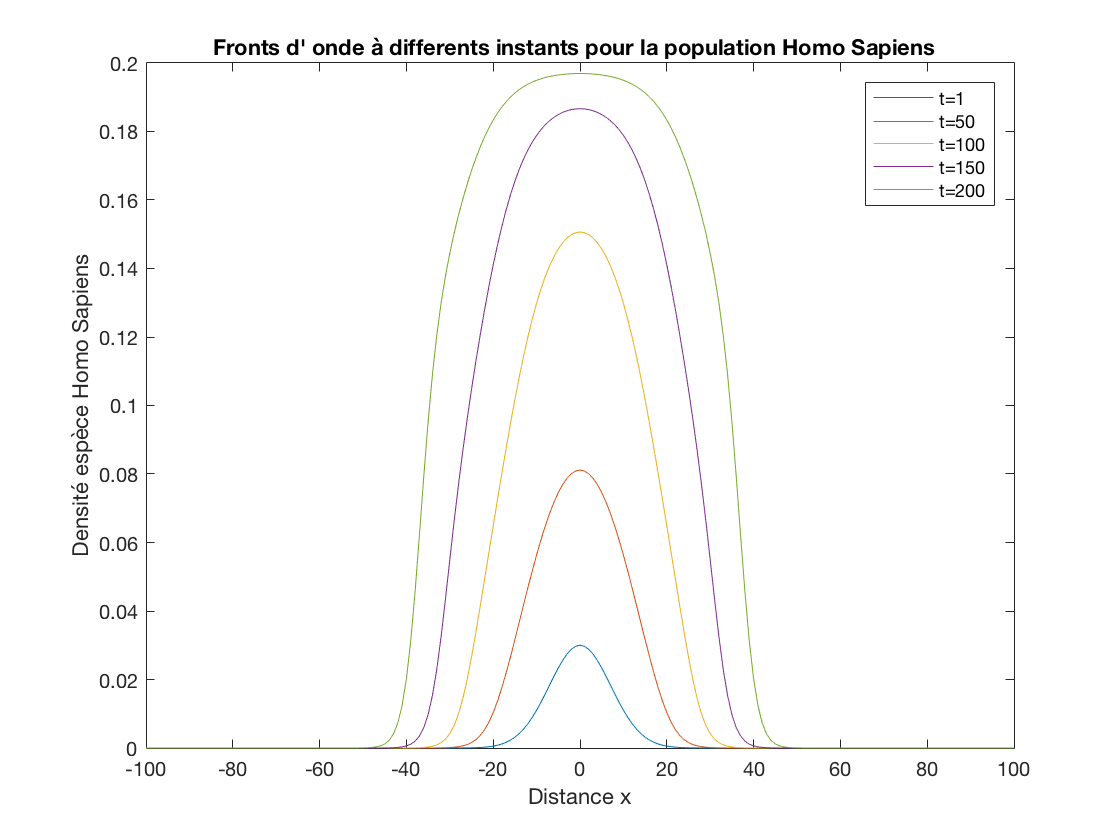
\includegraphics[width=0.48\linewidth]{Comp/homo.png}
\caption{Evolution des fronts d'onde au cours du temps}
\end{figure}
\end{frame}

\begin{frame}{Simulations Numériques}{Système de Lotka Volterra}
\begin{figure}[H]
\centering
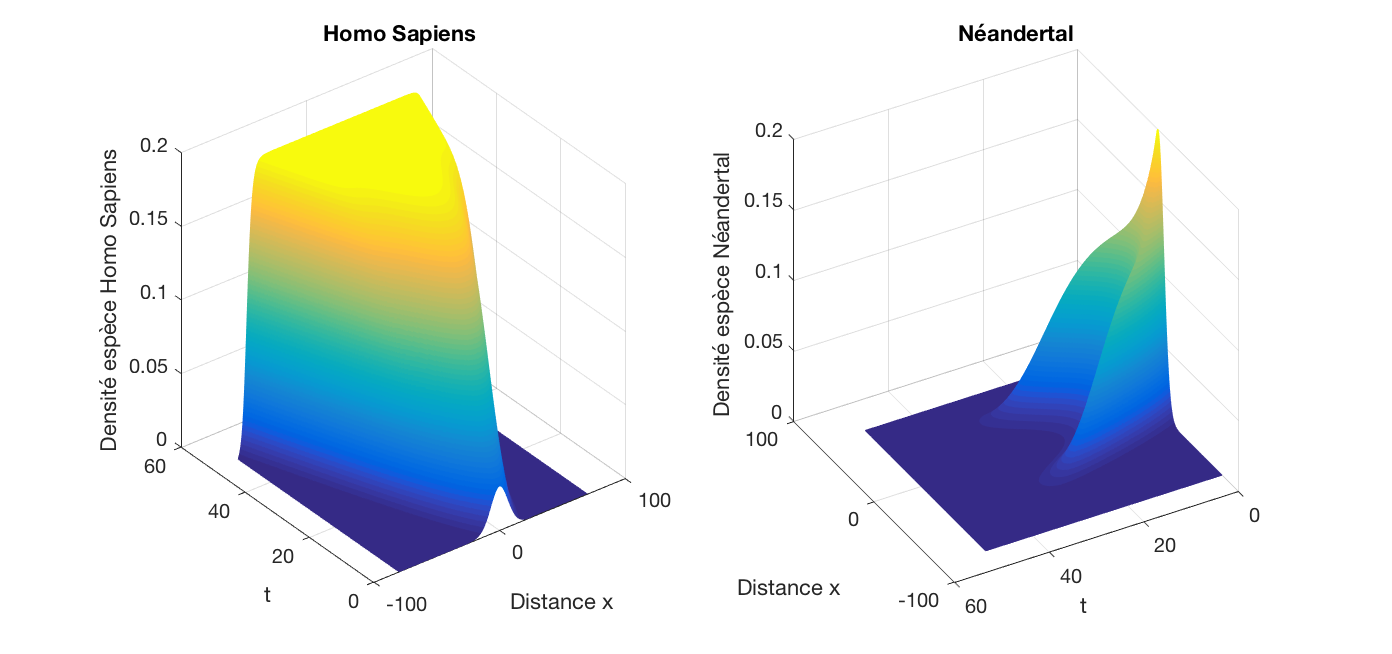
\includegraphics[scale=0.2]{Comp/CompDiff2.png}
\caption{Diffusion 1D}
\end{figure}
\end{frame}


\end{document}